\section{Improve a Proactive}
	\subsection{Reason to Choose}
		

	\subsection{SMART}
		\begin{SMART}
		    \item[Specific] A proactive for me is to be present and on time. That's one of my biggest weaknesses.
		    \item[Measurable] This can be measured by a statistical comparison of the times when I was on time and unpunctual. In addition, you can compare my arrival and absent-ness percentage together.
		    \item[Attainable] In the present time appointments, work schedules and events are an integral part and therefore time management is a very important issue.
		    \item[Relevant] This is a very relevant issue, as it could cost me my job if I am too often absent or late.
		    \item[Time-limited] The semester ends in January 2016 which is why I will have reached my goal by the end of January.
		\end{SMART}
	
	\subsection{STAR}
		\begin{STAR}
		    \item[Situation] 
		    \item[Task] 
		    \item[Action] 
		    \item[Result] 
		\end{STAR}
		
		\begin{figure}[htbp]
			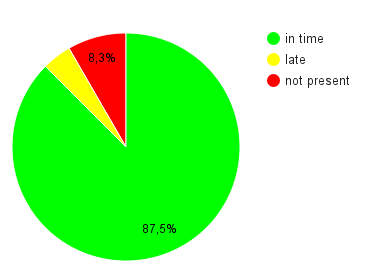
\includegraphics[width=\textwidth]{../img/inTimeDiagramm}
		\end{figure}